%!TEX root = ../../tcc.tex

\newpage
\section{Jogo da troca de arquivos}
\label{sec:titfortat}
\todo[inline]{arrumar uso dos termos choke/unchoke}

Nesta altura do processo de download de um \gls*{torrent}, o Transmission já realizou
muitos procedimentos. Tudo começou com a adição de um \gls*{torrentfile} ao programa,
que leu seus dados e identificou os endereços de \glspl*{tracker}; então, entrou em
contato com eles, que respondeu com uma lista de \glspl*{peer} que já estão no
\gls*{swarm}. Ou seja, até agora, não foi baixado nenhum byte sequer do arquivo contido
no pacote do \gls*{torrent}.

O BitTorrent trata a troca de dados entre \glspl*{peer} como um jogo que, usufruindo
das lógicas existentes na teoria dos jogos - área da matemática que estuda modelos
matemáticos de conflito e cooperação entre agentes inteligentes que tomam decisões -
, tenta se tornar um ambiente na qual se buscará as melhores condições de velocidades
de download e upload de arquivos e maior tempo de disponibilidade do \gls*{torrent} na
rede. Para isso, existe o conceito \emph{tit-for-tat} (olho por olho), que move o
BitTorrent de uma maneira geral: um \gls*{peer} preferirá ajudar \glspl*{peer} que o
ajudam, ou seja, só fará upload de partes para aqueles que o fizerem de volta.

Nesta seção, mostraremos o protocolo de mensagens para trocas de arquivos entre esses
\glspl*{peer} dessa lista e os algoritmos do BitTorrent dessas trocas.

%!TEX root = ../../tcc.tex

\subsection*{Estados dos nós e informações}

Existem 2 características independentes que formam as possibilidades de estados que um
\gls*{peer} pode assumir enquanto participa de um \gls*{swarm}:

\begin{itemize}
    \item \textbf{choking} (estrangulamento): se um \gls*{peer} \textbf{A} estrangulará
        a conexão com outro \gls*{peer} \textbf{B} (\emph{choked}) ou a deixará normal
        (\emph{unchoked}).

    \item \textbf{interested} (interesse): se um \gls*{peer} \textbf{A} terá interesse
        em um \gls*{peer} \textbf{B} (\emph{interested}) ou não (\emph{not interested})
\end{itemize}

Uma nova conexão entre \glspl*{peer} inicia em \emph{choked} e \emph{not interested} em
ambos os sentidos, ou seja, com \textbf{A} e \textbf{B} estrangulando suas conexões
mutuamente e sem interesse no outro. Esses estados ditarão todas as estratégias de troca
de partes entre \glspl*{peer}.

Outra informação utilizada é o \emph{bitfield}, que é um mapa de bits onde cada bit
representa uma parte que o \gls*{peer} já possui.

%!TEX root = ../../tcc.tex

\subsection*{Mensagens}

O protocolo é definido por 12 mensagens e 2 tipos de assinaturas. Essas mensagens são
enviadas entre \glspl*{peer} e serve para estes tomarem conhecimento da situação de
download de um \gls*{torrent}. A primeira assinatura é exclusiva da mensagem de
handshake, enquanto todas as outras seguem o mesmo padrão.

\subsubsection*{handshake}

assinatura: \bverb|<tam. header><header><bytes reservados><info_hash><peer_id>|

O \emph{handshake} (aperto de mãos) é a primeira mensagem a ser enviada por um
\gls*{peer} que recém-chegado à rede.

\begin{itemize}
    \item \bverb|<tam. header>|: tamanho da string \bverb|<header>|,
        representado em binário por 1 byte. O comprimento oficial é 19.

    \item \bverb|<header>|: \gls*{string} identificadora do protocolo. Na versão 1.0 do
        protocolo BitTorrent, a \gls*{string} oficial é \sverb|BitTorrent protocol|.

    \item \bverb|<bytes reservados>|: seção de 8 bytes (= 64 bits) reservados para a
        habilitação de funcionalidades extras do protocolo. Um e-mail enviado pelo
        criador do BitTorrent Bram Cohen \cite{wikitheory:reserved-bytes} sugere que os
        bits menos significativos sejam usados primeiro, para que os mais significativos
        possam ser usados para alterar o significado dos bits finais. A implementação de
        cada uma das funcionalidades não-oficiais depende do programa cliente. A tabela
        abaixo mostra os bits e seus respectivos usos, oficiais (*) ou não-oficiais.

        \begin{center}
            \begin{tabular}{ | c | c |}
            \hline
            \textbf{Bit} & \textbf{Uso}                         \\ \hline
            1       & Azureus Extended Messaging                \\ \hline
            1-16    & BitComet Extension protocol               \\ \hline
            21      & BitTorrent Location-aware Protocol 1.0    \\ \hline
            44      & Extension protocol                        \\ \hline
            47-48   & Extension Negotiation Protocol            \\ \hline
            61      & NAT Traversal                             \\ \hline
            62      & Fast Peers*                               \\ \hline
            63      & XBT Peer Exchange                         \\ \hline
            64      & DHT* ou XBT Metadata Exchange             \\ \hline
            \end{tabular}
        \end{center}

    \item \bverb|<info_hash>|: o ID do \gls*{torrent}, que é a \gls*{string}
        \gls*{hashvalue} de 20 bytes resultante da \gls*{hashfunction} SHA-1, com
        \gls*{urlencode}, do valor da chave \bverb|info| do arquivo \gls*{torrentfile};

    \item \bverb|<peer_id>|: ID único do cliente, que é uma \gls*{string} de 20 bytes,
        geralmente sendo o mesmo valor \bverb|peer_id| enviado nas requisições ao
        \gls*{tracker}, prefixado pelas informações como o nome do programa cliente e a
        sua versão. Por exemplo, o Transmission envia o prefixo \sverb|-TR2820-...|
\end{itemize}

\cfile[label="./libtransmission/handshake.c:191"]{./Codes/chap3/028-handshake.c}

Esse mensagem é enviada imediatamente pelo \gls*{peer} que inicia uma conexão. O
receptor deve responder, assim que ver o ID do \gls*{torrent} na seção de
\bverb|info_hash| da mensagem, com o seu \bverb|peer_id|. A conexão deve ser fechada em
dois casos: pelo receptor, se ele receber a mensagem para um ID de \gls*{torrent}
desconhecido para si, ou pelo iniciador, caso o \bverb|peer_id| recebido como resposta
seja diferente daquele indicado na lista de \glspl*{peer} recebida do \gls*{dht}.

\subsubsection*{keep-alive}

keep-alive: \bverb|<tamanho=0000>|

A mensagem de \emph{keep-alive} (``mantenha vivo'' em português literal) serve para
manter uma conexão aberta caso nenhuma outra mensagem seja enviada num período de tempo
(geralmente, 2 minutos).

Assim como as outras mensagens, esta mensagem usa a assinatura

\bverb|<tamanho><ID da mensagem><dados>|

\begin{itemize}
    \item \bverb|<tamanho>|: valor de 4 bytes em \emph{big} \gls{endian}

    \item \bverb|<ID da mensagem>|: decimal de 1 byte

    \item \bverb|<dados>|: dados a serem enviados ao outro \gls*{peer}, dependente da
        mensagem
\end{itemize}

Porém, não possui ID da mensagem nem dados a serem enviados, possuindo tamanho 0.

\cfile[label="./libtransmission/peer-msgs.c:1093"]{./Codes/chap3/029-keepalive.c}

\subsubsection*{choke e unchoke}

\hspace*{-\parindent} % alinha a tabela à margem esquerda
\begin{tabular}{r l}
choke: & \bverb|<tamanho=0001><ID da mensagem=0>| \\
unchoke: & \bverb|<tamanho=0001><ID da mensagem=1>|
\end{tabular}

Estas mensagens servem para indicar que a mudança de estado de choking que o \gls*{peer}
remetente tratará o receptor. Ou seja, o receptor \emph{choked} não terá suas
requisições atendidas, ao contrário de quando estiver \emph{unchoked}.

\cfile[label="./libtransmission/peer-msgs.c:431"]{./Codes/chap3/030-choke-unchoke.c}

\subsubsection*{interested e not interested}

\hspace*{-\parindent} % alinha a tabela à margem esquerda
\begin{tabular}{r l}
interested: & \bverb|<tamanho=0001><ID da mensagem=2>| \\
not interested: & \bverb|<tamanho=0001><ID da mensagem=3>|
\end{tabular}

Assim como as mensagens de \emph{choke}, estas 2 mensagens também servem para indicar a
mudança de estado, desta vez sendo a mudança de interesse que o \gls*{peer} remetente
terá no receptor.

\cfile[label="./libtransmission/peer-msgs.c:769"]{./Codes/chap3/031-interest.c}

\subsubsection*{have}

have: \bverb|<tamanho=0005><ID da mensagem=4><dados=i-ésima parte>|

A definição é que esta mensagem avisa um \gls*{peer} que a $i$-ésima parte do
\gls*{torrent} foi baixada pelo remetente e verificada através de \gls*{hashvalue}.
Porém, não necessariamente é usada dessa forma.

\cfile[label="./libtransmission/peer-msgs.c:399"]{./Codes/chap3/032-have.c}

Uma implementação de algoritmo do jogo da troca pode fazer com que um \gls*{peer}, que
acabou de adquirir a parte, não emitir aviso para todos os \gls*{peers} vizinhos que já
a possuem, diminuindo o \gls{overhead} de mensagens do protocolo. Por outro lado, enviar
esse aviso pode ajudar na determinação de qual parte é mais rara.

\subsubsection*{bitfield}

bitfield: \bverb|<tamanho=0001+X><ID da mensagem=5><dados=mapa de bits>|

O BitTorrent usa bitfields (mapas de bits) em \emph{big} \gls*{endian} para representar
na forma de \emph{flags} quais partes de um \gls*{torrent} já possui.

Esta mensagem só deve ser enviada imediatamente após o processo de \emph{handshake}
terminar e antes de qualquer outra mensagem. Se o \gls*{peer} não tiver nenhuma parte o
campo de dados pode ser omitido. Como bitfields variam de acordo com o tamanho total do
\gls*{torrent}, o comprimento da mensagem é variável, onde $X$ é o comprimento do
bitfield, acrescentado de alguns bits 0 de sobra no seu final (\emph{spare bits}).

Um bitfield de comprimento errado ou sem bits de sobra no final são considerados erros,
fazendo com que as respectivas conexões devam ser fechadas.

\cfile[label="./libtransmission/peer-msgs.c:2120"]{./Codes/chap3/033-bitfield.c}

\subsubsection*{request}

request: \bverb|<tamanho=0013><ID da mensagem=6><dados=<índice><início><tamanho>>|

Conforme foi explicado anteriormente (página \pageref{subsec:partes}), um
\gls*{torrent} divide os dados em partes. Porém, a transmissão não se dá enviando
partes inteiras, mas sim em blocos, que são metades das partes.

\begin{figure}[H]
    \centering
    \fbox{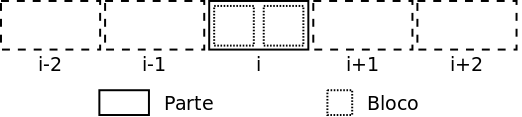
\includegraphics[width=0.64\textwidth]{partes.png}}
    \caption{trecho da seção de dados do torrent, com as divisões das partes e dos
    blocos}
    \label{fig:partes}
\end{figure}

Com esta mensagem, um \gls*{peer} pede por uma parte do \gls*{torrent}. A seção de dados
contém os seguintes números inteiros:

\begin{figure}[ht!]
    \centering
    \fbox{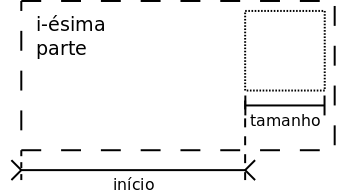
\includegraphics[width=0.64\textwidth]{request.png}}
    \caption{parâmetros da mensagem \emph{request} e seus significados}
    \label{fig:request}
\end{figure}

\begin{itemize}
    \item índice: índice da parte base $i$
    \item início: deslocamento, em bytes, da posição do bloco da parte $i$ pedido
    \item tamanho: tamanho, em bytes, do bloco pedido
\end{itemize}

\subsubsection*{piece}

piece: \bverb|<tamanho=0009+X><ID da mensagem=7><dados=<índice><início><bloco>>|

Esta mensagem é a resposta para a requisição de um bloco por meio da mensagem
\emph{request}, tendo assinatura análoga com exceção do trecho com os dados do bloco.
Assim, um \gls*{peer} envia um bloco de dados a outro.

O tamanho da mensagem é variável, onde $X$ é o tamanho do segmento de dados, já que
este pode ter tamanhos diferentes entre mensagens diferentes. A seção de dados possui
os seguintes números inteiros:

\begin{itemize}
    \item índice: índice da parte base $i$
    \item início: deslocamento, em bytes, da posição do bloco da parte $i$ pedido
    \item bloco: conteúdo dos dados do bloco
\end{itemize}

\subsubsection*{cancel}

cancel: \bverb|<tamanho=0013><ID da mensagem=8><dados=<índice><início><tamanho>>|

A mensagem \emph{cancel} serve para cancelar a mensagem \emph{request} de mesmos
parâmetros. É mais utilizada durante o algoritmo de fim de jogo.

\todo[inline]{referenciar seção do algoritmo do fim de jogo}

\subsubsection*{port}

cancel: \bverb|<tamanho=0003><ID da mensagem=9><dados=porta>|

Para os casos do \gls*{peer} estar usando a função de \gls*{dht}, esta mensagem serve
para avisar ao receptor qual a porta de comunicação \gls*{tcp} que o remetente está
usando para receber mensagens de \gls*{dht}; Com isso, é adicionado à tabela de
roteamento do receptor.

%!TEX root = ../../tcc.tex

\newpage
\subsection*{Algoritmos de seleção de partes}

Por se tratar de um protocolo de troca de dados em partes, uma escolha ruim de quais
destas se adquirir primeiro faz com que seja grande a possibilidade de um \gls*{peer}
baixar alguma parte que seja sempre ofertada por outros \glspl*{peer}. Isso acarretará
em não se ter nenhuma das partes que se deseja. Assim, durante a troca das partes, um
\gls*{peer} adota estratégias diferentes para fornecer e receber blocos de dados, com o
intuito de tentar otimizar a obtenção do conjunto total de dados dos \glspl*{torrent} e
ajudando a difundir o conteúdo deste ao resto do \gls*{swarm}.

As estratégias a seguir são medidas que um \gls*{peer} BitTorrent pode adotar com
efeitos em si mesmo, sem afetar outros \glspl*{peer}.

\subsubsection*{Random First Piece}

No início do download de um \gls*{torrent}, um \gls*{peer} não possui partes. Para que
comece a receber partes, ele avisa que é recém-chegado, e assim algum membro do
\gls*{swarm} envia-no uma parte comum aleatoriamente. Dessa forma, ele possuirá uma
``moeda de troca'', podendo então ajudar outros \glspl*{peer} e, assim, conseguirá
melhores condições de ser atendido. É importante que a parte seja comum, pois assim
será possível conseguir blocos de locais diferentes; se fosse rara, seria mais difícil
conseguir completá-la

Após completar a primeira parte, o algoritmo passa para a estratégia de \emph{Rarest
First}.

\subsubsection*{Rarest First}

Nesta fase, o \gls*{peer} passa a pedir as partes mais raras antes. Para isso, utiliza
os bitfields recebidos dos outros \glspl*{peer}, mantendo-os atualizados a cada mensagem
\bverb|have| que recebe. Feito isso, das partes que são menos frequentes nos bifields,
escolhe uma aleatoriamente, devido ao fato de que uma parte rara poderia ser muito
requisitada, o que seria improdutivo. Da mesma forma, a estratégia de deixar partes mais
comuns para serem baixadas mais tarde não é prejudicial, pois a probabilidade de que um
\gls*{peer} que está disponibilizando essas partes num dado momento deixará de ser
interessante é reduzida.

É fácil ver que, enquanto um \gls*{seeder} não enviar todas as partes do \gls*{torrent}
que está fornecendo, não haverá nenhum \gls*{peer} que possa ter terminado de baixá-lo.
Assim, quando o \gls*{seeder} possuir capacidade de upload menor do que de seus
\glspl*{leecher}, a melhor situação será se cada um destes baixar partes diferentes dos
outros, que maximiza o espalhamento dos dados e alivia a carga sobre o \gls*{seeder},
justificando a prioridade em se fazer download das partes raras.

Em uma outra situação, o \gls*{seeder} pode sair da rede, tornando os \glspl*{leecher}
responsáveis pela distribuição do \gls*{torrent}. Assim, corre-se o risco de alguma
parte se tornar indisponível. O \emph{rarest first} também ajuda neste caso, pois
replica as partes raras o mais rápido possível, reduzindo o risco do \gls*{torrent} se
tornar incompleto.

\subsubsection*{Strict Priority}

Cada parte é composta de blocos, que são os pacotes de dados trocados entre
\glspl*{peer}. Esta política de prioridade faz com que, se um bloco for requisitado, o
restante dos blocos da mesma parte serão pedidos antes dos blocos de outras partes, a
fim de se ter partes completas o mais rápido possível.

\subsubsection*{Endgame Mode}

Próximo ao fim do download de um \gls*{torrent}, a tendência é que os últimos blocos de
dados demorem, chegando aos poucos. Para agilizar isso, o cliente pede todos os blocos
faltantes para todos os \glspl*{peer}, enviando uma mensagem \bverb|cancel| para todos
que não tiverem respondido à requisição assim que o bloco é recebido para evitar
despedício de banda de rede na recepção redundante de dados.

\subsubsection*{Implementação do Transmission}

O Transmission implementa as partes desejadas e os blocos do \gls*{torrent} a serem
baixados como vetores. O vetor de partes é ordenado, utilizando seus campos auxiliares,
de forma que a parte mais importante que se deseja receber será requisitada antes. Ele
é usado para decidir quais blocos serão requisitados.

\cfile[label="./libtransmission/peer-mgr.c:167"]{./Codes/chap3/038-struct-weighted-piece.c}

Conforme são recebidas mensagens \bverb|have| e \bverb|bitfield| de outros \glspl*{peer},
ocorre o processamente da carga de dados dessas mensagens e a atualização das
informações das partes de cada remetente. Assim, o Transmission estima quais partes do
\gls*{torrent} são mais raras que outras, guardando essa informação no vetor de
replicações.

\cfile[label="./libtransmission/peer-mgr.c:1699"]{./Codes/chap3/041-peer-callback.c}

Já o vetor de blocos mantém a lista dos blocos pedidos com o momento da requisição e
para quem o foi feito. É usada para cancelar requisições que ficaram pendentes por muito
tempo ou para evitar requisições duplicadas antes do modo de fim de jogo.

\cfile[label="./libtransmission/peer-mgr.c:161"]{./Codes/chap3/039-struct-block-request.c}

Ambos os vetores são armazenados em uma estrutura que guarda essas e outras informações
sobre o \gls*{swarm} do \gls*{torrent} que está sendo baixado.

\cfile[label="./libtransmission/peer-mgr.c:178"]{./Codes/chap3/040-struct-swarm.c}

Eventualmente, o Transmission verifica a necessidade e a capacidade de enviar pedidos
de blocos. Caso seja possível, realiza o processamento da lista de partes, montando uma
lista de blocos a serem requisitados.

\newpage
\cfile[label="./libtransmission/peer-mgr.c:1324"]{./Codes/chap3/042-peer-mgr-getreqs.c}

\newpage
Tendo criado a lista de blocos, os requisita.

\cfile[label="./libtransmission/peer-msgs.c:1874"]{./Codes/chap3/043-update-block-reqs.c}

%!TEX root = ../../tcc.tex

\newpage
\subsection*{Algoritmos de enforcamento}

Além das estratégias mostradas, existem as estratégias que são as formas com que um
\gls*{peer} se relacionará com seus vizinhos. Cada um é responsável por melhorar as
suas taxas de download e, para isso, baixam partes de quem eles conseguem e escolhem se
para quais enviará outras, de forma a mostrar cooperação. Caso a escolha seja de não
cooperar, um \gls*{peer} enforca (\emph{choke}) outro, que implica num cancelamento
temporário do envio de partes para ele. O recebimento de partes continua normalmente e a
conexão não precisa ser rediscutida quando o enforcamento terminar.

O choking não faz parte do protocolo de mensagens, mas é necessário para a boa
performance do protocolo. Um bom algoritmo de choking, que utilize de todos os recursos
disponíveis, traz boas condições para todos os \glspl*{peer} cooperativos e é resistente
contra aqueles que só fazem download.

\subsubsection*{Eficiência de Pareto}

Sistemas \emph{pareto eficientes} \cite{wiki:pareto} são aqueles onde duas entidades
não podem fazer trocas e ficar mais ``felizes'' que antes. Em termos da Ciência da
Computação, buscar a eficiência de Pareto é usar um algoritmo de otimização local onde
as entidades procuram meios de melhorar mutuamente, que convergem a uma situação ótima
global. No contexto do BitTorrent, se 2 \glspl*{peer} não estão tendo vantagem
recíproca por enviar partes, eles podem começar a trocar partes entre si e conseguir
taxas de download melhores do que as anteriores.

\subsubsection*{Algoritmo de choking}

Cada \gls*{peer} sempre fará unchoke de 4 \glspl*{peer} (geralmente), então o problema
passa ser escolher quais deles fazer, deixando que o \gls*{tcp} controle de
congestionamento de banda. Essa escolha é baseada estritamente na taxa de download,
calculando a média dessa taxa durante 20 segundos. Antigamente, esse cálculo era feito
sobre quantidades transferidas a longos prazos, mas notou-se que era uma medida fraca
por causa das variações da largura da banda de rede.

Para evitar que recursos sejam desperdiçados pelo rápido choke e unchoke de
\glspl*{peer}, um cálculo é realizado a cada 10 segundos a fim de saber quem sofrerá o
choke, deixando a situação atual como está até o próximo intervalo acabar. Esse tempo é
suficiente para que o \gls*{tcp} acelere transferências até sua capacidade total.

\subsubsection*{Optimistic Unchoking}

Fazer upload para \glspl*{peer} que possuem as melhores taxas de download sofrem do fato
de não possuir meios de descoberta de conexões melhores. Para tentar contornar esse
problema, um \gls*{peer} será escolhido para ser alvo de um ``unchoke otimista'', que é
um unchoke independentemente da taxa de download que ele provê.

A escolha do \gls*{peer} ocorre a cada 30 segundos (no terceiro ciclo de choke), que é
tempo suficiente para o upload chegar à velocidade máxima, um download ocorrer como
recompensa e chegar à sua velocidade máxima.

Este algoritmo tem como objetivo demonstrar cooperação, sendo equivalente a demonstrar
colaboração como iniciativa num caso de jogo do tipo dilema do prisioneiro.

\subsubsection*{Anti-snubbing}

Eventualmente, um \gls*{peer} sofrerá choke de todos os \glspl*{peer} de onde estava
fazendo download. Nesses casos, terá taxas de download ruims até que um unchoke
otimista seja executado.

Quando ficar mais de 1 minuto sem ter recebido nenhuma parte de outro \gls*{peer}, o
\gls*{peer} que não recebeu nada perceberá que foi censurado (\emph{snubbed}), e
retaliará deixando de enviar partes para ele a menos que tenha sido por sorteio de
um unchoke otimista. Dessa forma, vários unchokes otimistas serão executados
simultaneamente, que implicará na recuperação das taxas de download.

\subsubsection*{Upload Only}

Uma vez que um \gls*{peer} terminou de baixar os dados do \gls*{torrent}, ele não
precisa mais escolher para quem fará o upload usando sua taxa de download. Ao invés
disso, passará a enviar dados para os \glspl*{peer} com quem possui as maiores taxas de
upload, que são os que não estão recebendo muitos dados, então utilizando toda a sua capacidade de upload.

\subsubsection*{Implementação do Transmission}

Quando um \gls*{torrent} é executado e em intervalos de 10 segundos, o Transmission
executa uma função que faz os chokes de upload e também verifica os downloads.

\cfile[label="./libtransmission/peer-mgr.c:3167"]{./Codes/chap3/047-rechoke-pulse.c}

Primeiro, verifica os uploads. A cada execução da função, verifica se será um turno de
unchoke otimista, que dura 4 execuções. Além disso, o vetor de \glspl*{peer} é usado
para o carregamento de um vetor temporário de informações para choke sobre cada um
deles.

\cfile[label="./libtransmission/peer-mgr.c:3057"]{./Codes/chap3/048-rechoke-up1.c}

A ordenação é feita com \sverb|qsort()| usando uma função comparadora que classifica os
\glspl*{peer} considerando, nesta ordem:

\begin{enumerate}
    \item velocidade de transferência de dados (download e upload)
    \item estado de choke: preferência por unchoked
    \item aleatoriedade
\end{enumerate}

\cfile[label="./libtransmission/peer-mgr.c:2993"]{./Codes/chap3/049-compare-choke.c}

Então, trata o vetor temporário. Os melhores \glspl*{peer} mudarão seu estado para
unchoked, enquanto o resto será choked. Além disso, no caso de um rodada de unchoke
otimista, sorteia um dos \glspl*{peer} para ter a sua vez.

\cfile[label="./libtransmission/peer-mgr.c:3057"]{./Codes/chap3/050-rechoke-up2.c}

Depois, trata os downloads. Primeiro, calcula para quantos \glspl*{peer} mandar
mensagens \bverb|interested| usando como base as estatísticas de pedidos de blocos e
quais deles foram cancelados, dentro de limites de bom funcionamento.

\cfile[label="./libtransmission/peer-mgr.c:2833"]{./Codes/chap3/051-rechoke-down1.c}

Após saber o limite de \glspl*{peer}, o Transmission procura quais deles contatará, de
acordo com as partes que lhe faltam. Para isso, monta um vetor com informações dos
\glspl*{peer}, ordenando usando \sverb|qsort()| e passando como função comparadora que
avalia, nesta ordem:

\begin{enumerate}
    \item estado de choke: se um \gls*{peer} tiver cancelado 10\% ou menos dos pedidos
        de blocos, terá preferência sobre os outros.
    \item aleatoriedade.
\end{enumerate}

\cfile[label="./libtransmission/peer-mgr.c:2813"]{./Codes/chap3/053-enum-rechoke.c}

\cfile[label="./libtransmission/peer-mgr.c:2820"]{./Codes/chap3/052-compare-rechoke.c}

\cfile[label="./libtransmission/peer-mgr.c:2833"]{./Codes/chap3/054-rechoke-down2.c}